\chapter{Forschungsmethodik}
Als Forschungsmethode wird in dieser Arbeit ``The Human-Centered Design Process'' (menschenzentriertes Design) nach \citeauthor{Norman13} angewandt. \\
Dieser definiert jenen Prozess in seinem Buch ``The Design of Everyday Things: Revised and Expanded Version'' wie folgt: \citep[Abbildung 6.2]{Norman13}

\begin{quote}
  ``Make observations on the intended target population, generate ideas, produce prototypes and test them.
  Repeat until satisfied.''
\end{quote}

\noindent
Die Idee des ``Human-Centered Design Process'' ist es, die durch Beobachtung einer zielgruppen-ähnlichen Menge an Test-Personen identifizierten Usability-Probleme iterativ zu lösen.
Hierzu beschreibt \citeauthor{Norman13} den Prozess als Zyklus, welcher sich aus vier Phasen zusammensetzt.
Dieser Zyklus wird iterativ so lange wiederholt, bis sich in der Testphase keine weiteren Usability-Probleme mehr identifizieren lassen, oder man mit den bis dahin erzielten Ergebnissen zufrieden ist. \\

\begin{figure}[h]
  \centering
  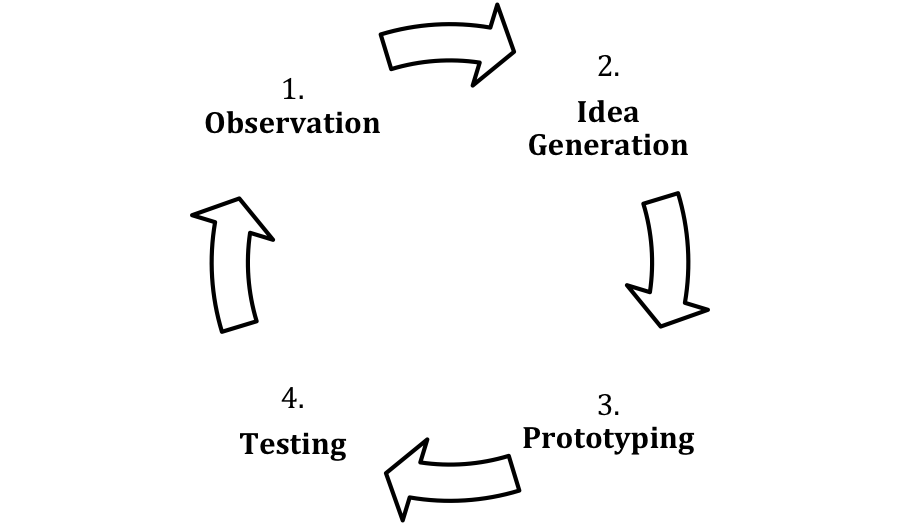
\includegraphics[keepaspectratio]{hcp}
  \caption{The Human-Centered Design Process}
  \label{fig:hcp}
\end{figure}

\noindent
In \autoref{fig:hcp} sieht man die vier verschiedenen Phasen des Zyklus:
\begin{enumerate}
  \item Observation (Beobachtung) \label{itm:observation}
  \item Idea Generation (Ideenfindung) \label{itm:idea}
  \item Prototyping (Prototypenentwicklung) \label{itm:prototyping}
  \item Testing (Testen) \label{itm:testing}
\end{enumerate}

\noindent
Zu Beginn des Zyklus (Observation) wird eine Menge an Test-Personen ausgewählt, welche möglichst repräsentativ für die eigentliche Zielgruppe des Problems ist. 
Diese ausgewählte Test-Gruppe wird bei der Bearbeitung von Aufgaben, die für das Usability-Problem relevant sind, zu jeder Zeit beobachtet und eventuelle Probleme werden notiert. 
Auf diese Weise ist es den Beobachtern möglich, ein tiefgründiges Verständnis für die angestrebten Ziele und den dabei auftauchenden Problemen der Test-Personen zu erlangen. \\

In der zweiten Phase (Idea Generation) wird versucht möglichst viele Ideen zur Lösung der in der ersten Phase identifizierten Probleme zu finden.
Hierzu führt \citeauthor{Norman13} drei Regeln zur Orientierung an \citep[Seite 226]{Norman13}:

\begin{itemize}
  \item ``Generate numerous ideas'' (Generiere viele Ideen)
  \item ``Be creative without regard for constraints'' (Sei grenzenlos kreativ)
  \item ``Question everything'' (Hinterfrage alles)
\end{itemize}

\noindent
Zusammengefasst sagen diese drei Regeln aus, dass es bei der Ideenfindung (Idea generation) durchaus sinnvoll sein kann, sich nicht auf die Findung \textbf{der} optimalen Lösung für ein Problem zu versteifen, sondern möglichst viele, kreative Ideen zu sammeln, die zur finalen Lösung alle einen kleinen Anteil beitragen. \\

Anschließend werden in der dritten Phase (Prototyping) erste Lösungsansatze in Form von Mock-Ups oder Prototypen zu den Ideenn aus der vorherigen Phase entwickelt.
Diese Prototypen werden am Ende des Zyklus (Testing) einer ausgewählten Menge an Test-Personen zum Testen zur Verfügung gestellt. Bei der Auswertung dieser Tests erhofft man sich einen Großteil der in Phase 1 identifizierten Probleme zu lösen.
Es kann jedoch auch vorkommen, dass während dieses ganzes Prozesses Probleme bis zur letzten Phase unerkannt bleiben, oder durch die Lösung eines Problems ein Neues entsteht.
Diese neu gewonnenen Eindrücke werden dann mit in die nächste Iteration des Design-Prozesses genommen, und bestenfalls bei einem weiteren Durchlauf des Zyklus gelöst. \\

Das Ziel dieses Entwicklungsprozesses ist es, den Zyklus so lange zu wiederholen, bis sich optimalerweise keine Usability-Probleme mehr finden lassen. \\

